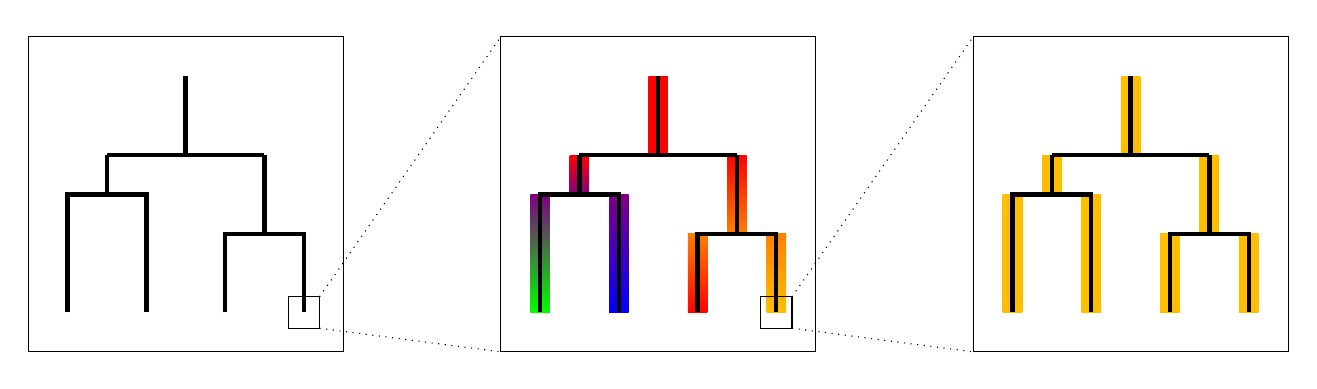
\begin{tikzpicture} 
  % Shade underneath left phylogeny
  % \shade[top color=red!100!yellow,bottom color=red!100!yellow] (0.5-0.124,6.0) rectangle (0.5+0.124,5.0);
  % \shade[top color=red!100!yellow,bottom color=red!50!blue] (-0.5-0.124,5.0) rectangle (-0.5+0.124,4.5);
  % \shade[top color=red!100!yellow,bottom color=red!50!yellow] ( 1.5-0.124,5.0) rectangle ( 1.5+0.124,4.0);

  % \shade[top color=red!50!blue,bottom color=red!0!green] (-1.0-0.124,4.5) rectangle (-1.0+0.124,3.0);
  % \shade[top color=red!50!blue,bottom color=blue!100!purple] ( 0.0-0.124,4.5) rectangle ( 0.0+0.124,3.0);
  % \shade[top color=red!50!yellow,bottom color=red!100!yellow] ( 1.0-0.124,4.0) rectangle ( 1.0+0.124,3.0);
  % \shade[top color=red!50!yellow,bottom color=red!25!yellow] ( 2.0-0.124,4.0) rectangle ( 2.0+0.124,3.0);
  % Left species phylogeny
  \draw[] (-1.5,2.5) rectangle (2.5,6.5); 
  \draw[ultra thick] ( 0.5,6.0) node {} -- ( 0.5,5.0) node {}; 
  \draw[ultra thick] (-0.5,5.0) node {} -- ( 1.5,5.0) node {}; 
  \draw[ultra thick] (-0.5,5.0) node {} -- (-0.5,4.5) node {}; 
  \draw[ultra thick] ( 1.5,5.0) node {} -- ( 1.5,4.0) node {}; 
  \draw[ultra thick] (-1.0,3.0) node {} -- (-1.0,4.5) node {} -- ( 0.0,4.5) node {} -- ( 0.0,3.0) node {}; 
  \draw[ultra thick] ( 1.0,3.0) node {} -- ( 1.0,4.0) node {} -- ( 2.0,4.0) node {} -- ( 2.0,3.0) node {}; 

  % Shade underneath middle phylogeny
  \shade[shift={(6 cm,0 cm)},top color=red!100!yellow,bottom color=red!100!yellow] (0.5-0.124,6.0) rectangle (0.5+0.124,5.0);
  \shade[shift={(6 cm,0 cm)},top color=red!100!yellow,bottom color=red!50!blue] (-0.5-0.124,5.0) rectangle (-0.5+0.124,4.5);
  \shade[shift={(6 cm,0 cm)},top color=red!100!yellow,bottom color=red!50!yellow] ( 1.5-0.124,5.0) rectangle ( 1.5+0.124,4.0);

  \shade[shift={(6 cm,0 cm)},top color=red!50!blue,bottom color=red!0!green] (-1.0-0.124,4.5) rectangle (-1.0+0.124,3.0);
  \shade[shift={(6 cm,0 cm)},top color=red!50!blue,bottom color=blue!100!purple] ( 0.0-0.124,4.5) rectangle ( 0.0+0.124,3.0);
  \shade[shift={(6 cm,0 cm)},top color=red!50!yellow,bottom color=red!100!yellow] ( 1.0-0.124,4.0) rectangle ( 1.0+0.124,3.0);
  \shade[shift={(6 cm,0 cm)},top color=red!50!yellow,bottom color=red!25!yellow] ( 2.0-0.124,4.0) rectangle ( 2.0+0.124,3.0);
  % Middle species phylogeny
  \draw[shift={(6 cm,0 cm)}] (-1.5,2.5) rectangle (2.5,6.5); 
  \draw[shift={(6 cm,0 cm)},ultra thick] ( 0.5,6.0) node {} -- ( 0.5,5.0) node {}; 
  \draw[shift={(6 cm,0 cm)},ultra thick] (-0.5,5.0) node {} -- ( 1.5,5.0) node {}; 
  \draw[shift={(6 cm,0 cm)},ultra thick] (-0.5,5.0) node {} -- (-0.5,4.5) node {}; 
  \draw[shift={(6 cm,0 cm)},ultra thick] ( 1.5,5.0) node {} -- ( 1.5,4.0) node {}; 
  \draw[shift={(6 cm,0 cm)},ultra thick] (-1.0,3.0) node {} -- (-1.0,4.5) node {} -- ( 0.0,4.5) node {} -- ( 0.0,3.0) node {}; 
  \draw[shift={(6 cm,0 cm)},ultra thick] ( 1.0,3.0) node {} -- ( 1.0,4.0) node {} -- ( 2.0,4.0) node {} -- ( 2.0,3.0) node {}; 
  % Zoomer between left and middle
  \draw[] (2.0-0.2,3.0-0.2) rectangle (2.0+0.2,3.0+0.2); 
  \draw[dotted] (2.0+0.2,3.0+0.2) node {} -- (4.5,6.5) node {}; 
  \draw[dotted] (2.0+0.2,3.0-0.2) node {} -- (4.5,2.5) node {}; 

  % Shade underneath right phylogeny
  \shade[shift={(12 cm,0 cm)},top color=red!25!yellow,bottom color=red!25!yellow] (0.5-0.124,6.0) rectangle (0.5+0.124,5.0);
  \shade[shift={(12 cm,0 cm)},top color=red!25!yellow,bottom color=red!25!yellow] (-0.5-0.124,5.0) rectangle (-0.5+0.124,4.5);
  \shade[shift={(12 cm,0 cm)},top color=red!25!yellow,bottom color=red!25!yellow] ( 1.5-0.124,5.0) rectangle ( 1.5+0.124,4.0);

  \shade[shift={(12 cm,0 cm)},top color=red!25!yellow,bottom color=red!25!yellow] (-1.0-0.124,4.5) rectangle (-1.0+0.124,3.0);
  \shade[shift={(12 cm,0 cm)},top color=red!25!yellow,bottom color=red!25!yellow] ( 0.0-0.124,4.5) rectangle ( 0.0+0.124,3.0);
  \shade[shift={(12 cm,0 cm)},top color=red!25!yellow,bottom color=red!25!yellow] ( 1.0-0.124,4.0) rectangle ( 1.0+0.124,3.0);
  \shade[shift={(12 cm,0 cm)},top color=red!25!yellow,bottom color=red!25!yellow] ( 2.0-0.124,4.0) rectangle ( 2.0+0.124,3.0);
  % Right species phylogeny
  \draw[shift={(12 cm,0 cm)}] (-1.5,2.5) rectangle (2.5,6.5); 
  \draw[shift={(12 cm,0 cm)},ultra thick] ( 0.5,6.0) node {} -- ( 0.5,5.0) node {}; 
  \draw[shift={(12 cm,0 cm)},ultra thick] (-0.5,5.0) node {} -- ( 1.5,5.0) node {}; 
  \draw[shift={(12 cm,0 cm)},ultra thick] (-0.5,5.0) node {} -- (-0.5,4.5) node {}; 
  \draw[shift={(12 cm,0 cm)},ultra thick] ( 1.5,5.0) node {} -- ( 1.5,4.0) node {}; 
  \draw[shift={(12 cm,0 cm)},ultra thick] (-1.0,3.0) node {} -- (-1.0,4.5) node {} -- ( 0.0,4.5) node {} -- ( 0.0,3.0) node {}; 
  \draw[shift={(12 cm,0 cm)},ultra thick] ( 1.0,3.0) node {} -- ( 1.0,4.0) node {} -- ( 2.0,4.0) node {} -- ( 2.0,3.0) node {}; 
  % Zoomer between middle and right
  \draw[shift={(6 cm,0 cm)}] (2.0-0.2,3.0-0.2) rectangle (2.0+0.2,3.0+0.2); 
  \draw[shift={(6 cm,0 cm)},dotted] (2.0+0.2,3.0+0.2) node {} -- (4.5,6.5) node {}; 
  \draw[shift={(6 cm,0 cm)},dotted] (2.0+0.2,3.0-0.2) node {} -- (4.5,2.5) node {}; 

\end{tikzpicture}